\section{Methodology} \label{sec:methodology}

\subsection{Granger causality and feedback} \label{sec:granger-causality}
Framework for causality testing was first proposed by Granger \cite{granger69} in 1969.
The original formulation had a general form with an example of a linear autoregressive model provided, further described in \fref{sec:linear-ar}.

Consider two time series $X_t$ and $Y_t$ of length $n$, which are assumed to be weakly stationary.
Lets denote an optimal, least-squares predictor of some time series $X_t$ given another time series $Y_t$ by $P_t(X|Y)$.
The residual errors of the model and its variance are defined as follows: 
$\varepsilon_t(X|Y) = X_t - P_t(X|Y)$ and $\sigma^2(X|Y) = var[\varepsilon_t(X|Y)]$.
Lastly, all available information until time $t$ will be denoted $U_t$.

Given such notation the following definitions are proposed:

\begin{definition} \label{def:causality}
	Causality

	If $\sigma^2(X|U) < \sigma^2(X|U-Y)$, then $Y_t$ causes $X_t$, denoted as $Y_t \Rightarrow X_t$.
\end{definition}
\begin{definition}
	Feedback

	If $\sigma^2(X|U) < \sigma^2(X|U-Y)$ and $\sigma^2(Y|U) < \sigma^2(Y|U-X)$, then there is feedback between $X_t$ and $Y_t$, denoted as $Y_t \Leftrightarrow X_t$.
\end{definition}

The completely unrealistic aspect of the formulation above is having access to the full information $U_t$.
In practice those definitions allow to construct statistical tests and to reason for causal relations between time series.

\subsubsection{Linear autoregressive model} \label{sec:linear-ar}
A simple realization of Granger causality test can be implemented using a two-variable linear autoregressive (AR) model of order $p$.
Two linear predictors of $X_t$ can be constructed as follows:

\begin{equation}
X_t = \sum_{i=1}^{p} \alpha_i X_{t-i} + \varepsilon_{X,t}
\end{equation}
\begin{equation}
X_t = \sum_{i=1}^{p} a_i X_{t-i} + \sum_{i=1}^{p} b_i Y_{t-i} + \varepsilon_{X|Y,t}
\end{equation}
where: $p$ is the order of AR model, $\alpha$, $a$, $b$ are scalar coefficients and $\varepsilon_{X,t}$, $\varepsilon_{X|Y,t}$ are residual errors of the models.
Causal relationship $Y_t \Rightarrow X_t$ can be inferred by comparing variance of residual errors $\varepsilon_{X,t}$ and $\varepsilon_{X|Y,t}$, as stated in \fref{def:causality} in \fref{sec:granger-causality}.

\subsubsection{Diks-Panchenko test}

To capture effects beyond linear causality nonparametric statistical tests are used.
In principle, such methods infer about some features of a system by constructing statistics on their distributions.
Those methods, not relying on a linear model, in context of Granger causality, are often called nonlinear Granger causality tests.
Diks and Panchenko \cite{diks-panchenko2004}, basing on earlier approaches by Hiemstra and Jones \cite{hiemstra-jones} and Baek and Brock \cite{baek-brock1992},
developed a test for nonlinear Granger causality.

Let $X_t^{l} = (X_t, X_{t-1}, \ldots X_{t-l+1})$ and $Y_t^{l} = (Y_t, Y_{t-1}, \ldots Y_{t-l+1})$
be lagged vectors of time series. The null hypothesis assumes no causality from $X_t \Rightarrow Y_t$:
\begin{equation} \label{eq:no-causality}
    Y_{t+1} | (X_t^{l}, Y_t^{l}) \sim Y_{t+1} | (Y_t^{l}) 
\end{equation}

Consider the following vector $W_t = (X_t^{l}, Y_t^{l}, Z_t)$ with $Z_t = Y_{t+1}$. \Fref{eq:no-causality} can be rewritten in terms of joint probability density function $f_{X,Y,Z}(x,y,z)$:
\begin{equation}
    \frac{f_{X,Y,Z}(x,y,z)}{f_Y(y)} = \
    \frac{f_{X,Y}(x,y)}{f_Y(y)} \frac{f_{Y,Z}(y,z)}{f_Y(y)}
\end{equation}

Next, the null hypothesis can be expressed as:
\begin{equation}
    q \equiv E [f_{X,Y,Z}(x,y,z) f_Y(y) - f_{X,Y}(x,y) f_{Y,Z}(y,z) ] = 0
\end{equation}

An estimator of $q$ based on indicator functions is:
\begin{equation}
    T_n(\varepsilon)= \
    \frac{(2\varepsilon)^{-d_X -2d_Y -d_Z}}{n(n-1)(n-2)} \
    \sum_i \
    \bigg[ \
    \sum_{k \neq i,j} \
    \sum_{j \neq i} \
    \Big( \
    I^{XYZ}_{ik} I^{Y}_{ij} - I^{XY}_{ik} I^{YZ}_{ij} \
    \Big) \
    \bigg]
\end{equation}
where $I^W_{ij}$ is the indicator function: $I^W_{ij} = I(||W_i-W_j||<\varepsilon)$, $I$ is equal to $1$ if the condition is met and $0$ otherwise,
$||\cdot||$ is the supremum norm,
$d_W$ is dimension of time series vector $W_t$,
$\varepsilon$ is bandwith.
   
Denoting local density estimator of random vector $W$ at $W_i$ as:
\begin{equation}
    \hat{f}_W(W_i)=\
    \frac{(2\varepsilon)^{-d_W}}{n-1}\
    \sum_{j,j \neq i} I^W_{ij}
\end{equation}
the test statistics is defined as follows:

\begin{equation} \label{eq:diks-panchenko-test}
    T_n(\varepsilon) = \
    \frac{(n-1)}{n(n-2)} \
    \sum_{i,j \neq i} \
    (\hat{f}_{X,Y,Z}(x,y,z) \
    \hat{f}_Y(y) - \
    \hat{f}_{X,Y}(x,y) \
    \hat{f}_{Y,Z}(y,z))
\end{equation}

It has been shown that the test is consistent for $\varepsilon = C n^{-\beta}$ for a positive constant $C$ and $\beta \in (\frac{1}{4}, \frac{1}{3})$ for sample size $n$.

\subsection{Wavelet transform} \label{sec:wavelet}
The term ``wavelet'' was coined by Grossmann and Morlet \cite{grossmann-morlet}  in the 1980s. 
The theory for this approach was further developed by many researchers, most notably Daubechies \cite{daubechies1990}.

A wavelet can be intuitively understood as a ``short, localized oscillation''.
The so-called mother wavelet, denoted as $\psi(t)$ is a function that satisfies the following conditions:

\begin{equation} \label{eq:wavelet-zero-mean}
	\int\! dt \: \psi (t) = 0
\end{equation}

\begin{equation} \label{eq:wavelet-norm}
	\int\! dt \: |\psi (t)|^2 = 1
\end{equation}
and the \emph{admissability condition}:
\begin{equation}
	\int\! d\omega \: |\omega|^{-1} \left(\mathscr{F} \psi\right)(\omega) < \infty
\end{equation}
where $\left(\mathscr{F} \psi\right)(\omega)$ is the Fourier transform of $\psi(t)$.

This function is then dilated and translated to account for frequency and localization:

\begin{equation}
	\psi^{(a,b)}(t) = \frac{1}{\sqrt{a}} \: \psi\left(\frac{t-b}{a}\right)
\end{equation}
The continuous wavelet transform $W(a,b)$ is a projection of the original signal $x(t)$ on the mother wavelet:

\begin{equation}
	W(a,b) = \int \! dt \: x(t) \psi^{(a,b)}(t)
\end{equation}

There are several widely used wavelet bases, typical examples are: Haar, Morlet, ``Mexican hat'' and Daubechies.
The mother wavelets of those examples are plotted on \fref{fig:wavelets}.

\begin{figure}[h]
	\centering
	\begin{subfigure}{\minipagewidth}
		\centering
		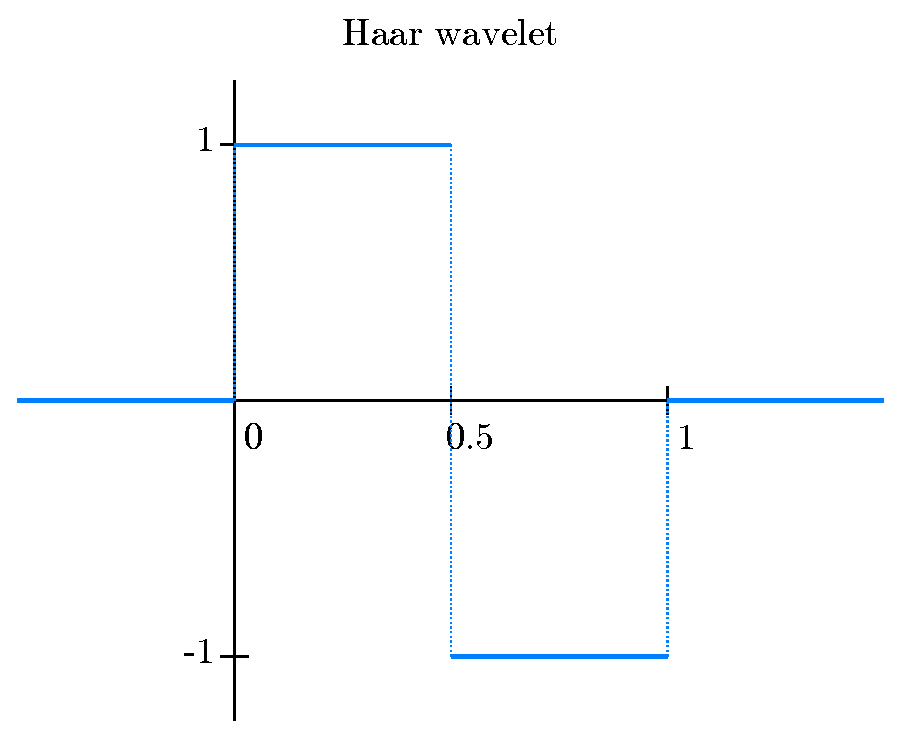
\includegraphics[width=\textwidth]{figures/haar.eps}
		\caption{}
	\end{subfigure}
	\begin{subfigure}{\minipagewidth}
		\centering
		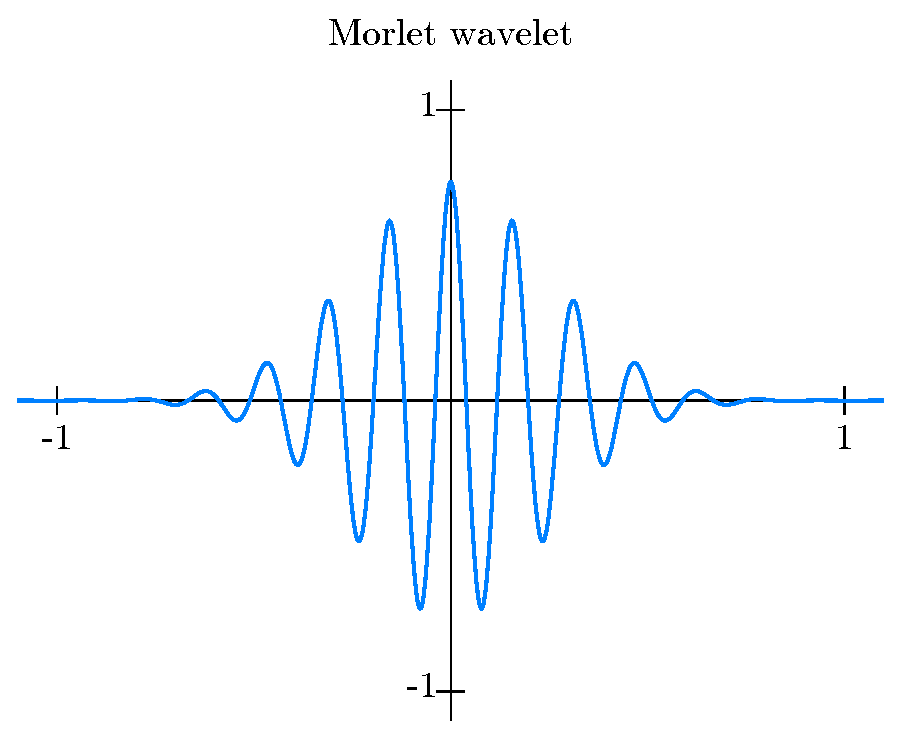
\includegraphics[width=\textwidth]{figures/morlet.eps}
		\caption{}
	\end{subfigure}
	\newline
	\begin{subfigure}{\minipagewidth}
		\centering
		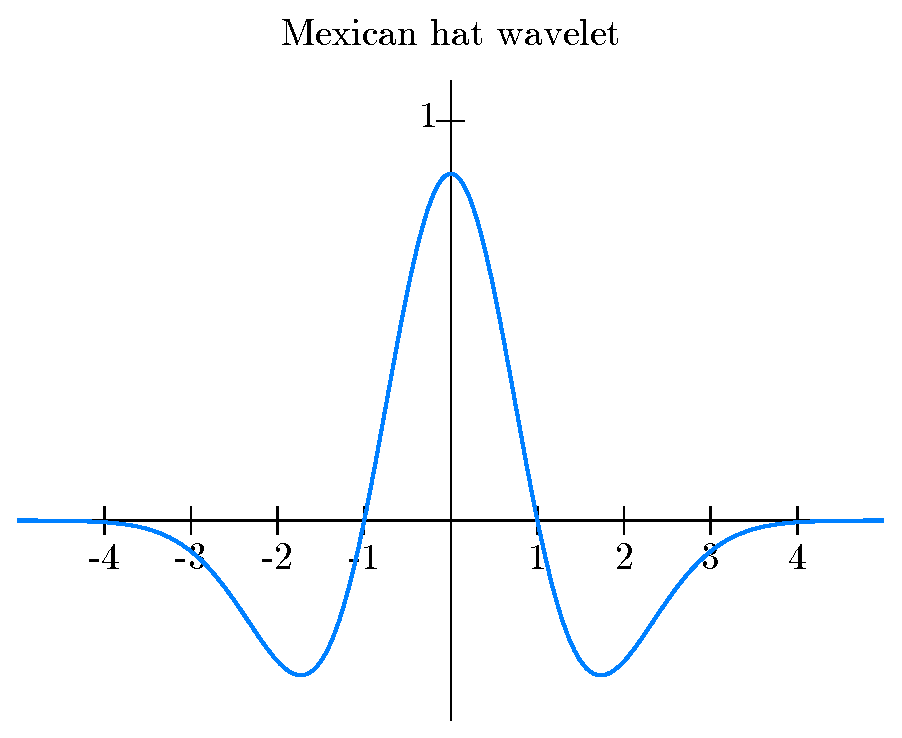
\includegraphics[width=\textwidth]{figures/mexican.eps}
		\caption{}
	\end{subfigure}
	\caption{Mother wavelets of (a) Haar (b) Morlet and (c) Mexican hat.}
	\label{fig:wavelets}
\end{figure}

\subsubsection{Discrete wavelet transform}
For practical purposes, to analyze real-life discrete time series, a discrete wavelet transform (DWT) is used.
It allows to decompose time series into multiple frequency scales.

The DWT is based on two discrete wavelet filters, called \emph{mother wavelet}
(which is a band-pass filter):
\begin{equation}
h_l=(h_0, h_1, \, \ldots \, h_{L-1})
\end{equation}
and \emph{father wavelet} (a low-pass filter):
\begin{equation}
g_l=(g_0, g_1, \, \ldots \, g_{L-1}).
\end{equation}
where $L$ is length of the filter.

In the disrete case, conditions \ref{eq:wavelet-zero-mean} and \ref{eq:wavelet-norm} for the mother wavelet become:

\begin{equation}
	\sum_{i=0}^{L-1} h_i = 0
\end{equation}

\begin{equation}
	\sum_{i=0}^{L-1} |h_i|^2 = 1.
\end{equation}
Additionally, $h_l$ is orthogonal to even shifts:

\begin{equation}
	\sum_{i=0}^{L-1} h_i h_{i+2n} = 0
\end{equation}
for all $n \neq 0$.

The father wavelet is constructed from the mother wavelet using the quadrature mirror relation:
\begin{equation}
	g_l = (-1)^{l+1} \:  h_{L-1-l}.
\end{equation}
Moreover, the scaling filter $g_l$ has the following properties:
\begin{center}
\noindent
\begin{minipage}[t]{\minipagewidth}
\begin{equation}
	\sum_{i=0}^{L-1} g_i = \sqrt{2},
\end{equation}
\end{minipage}
\begin{minipage}[t]{\minipagewidth}
\begin{equation}
	\sum_{i=0}^{L-1} |g_i|^2 = 1,
\end{equation}
\end{minipage}

\begin{minipage}[t]{\minipagewidth}
\begin{equation}
	\sum_{i=0}^{L-1} g_i g_{i+2n} = 0,
\end{equation}
\end{minipage}
\begin{minipage}[t]{\minipagewidth}
\begin{equation}
	\sum_{i=0}^{L-1} g_i h_{i+2n} = 0.
\end{equation}
\end{minipage}
\end{center}

In the discrete case dilations and translations of mother wavelet are expressed as:
$a=2^{-j}$ and $b=k 2^{-j}$, where $j, k \in \mathbb{N}$ and $j \leq J = log_2(T)$.
$J$ is the biggest number of scales and $T$ is the length of the time series.

To decompose a signal with DWT, a \emph{pyramid algorithm} is employed (see \fref{fig:pyramid}).
It consists of recursively applying low-pass and band-pass filters to the time series.
With each iteration of this scheme the high and low frequencies are separated.
The father wavelet captures the trend of the series, while mother wavelet extracts oscillatory components around the trend.

Let $w_i(t)$ represent the high frequency and $v_i(t)$ the low frequency of time series $X_t$ after $i$ iterations of the pyramid algorithm.
After the first pass one will get: $X_t = [w_1, v_1]$.
Then, applying this scheme again: $X_t = [w_1, w_2, v_2]$, and after $J$ iterations the time series will be decomposed into:
\begin{equation}
	X_t = [w_1, w_2, w_3, \, \dots \, w_J, v_J]
\end{equation}

\begin{figure}
\centering
\begin{tikzpicture}
% TOP RECTANGLES
	\draw[rounded corners] (0,0) rectangle ++(1.5,1) node[pos=0.5]{$X_t$};
	\draw[rounded corners] (3,0) rectangle ++(1.5,1) node[pos=0.5]{$v_1$};
	\draw[rounded corners] (6,0) rectangle ++(1.5,1) node[pos=0.5]{$v_2$};
	\draw[rounded corners] (11,0) rectangle ++(1.5,1) node[pos=0.5]{$v_J$};
% BOTTOM RECTANGLES
	\draw[rounded corners] (3,-2) rectangle ++(1.5,1) node[pos=0.5]{$w_1$};
	\draw[rounded corners] (6,-2) rectangle ++(1.5,1) node[pos=0.5]{$w_2$};
	\draw[rounded corners] (11,-2) rectangle ++(1.5,1) node[pos=0.5]{$w_J$};
% ARROWS
	\draw[thick, -{Latex}] (1.55,0.5) -- ++(1.4,0);
	\draw[thick, -{Latex}] (4.55,0.5) -- ++(1.4,0);
	\draw[thick, -{Latex}, dashed] (7.55,0.5) -- ++(3.4,0);

	\draw[thick, -{Latex}] (1.5,0) -- ++(1.5,-1.0);
	\draw[thick, -{Latex}] (4.5,0) -- ++(1.5,-1.0);
	\draw[thick, -{Latex}, dashed] (7.5,0) -- ++(3.5,-1.0);
% TEXT
	\node at (3.75,1.5) {$i=1$};
	\node at (6.75,1.5) {$i=2$};
	\node at (9.25,1.5) {$\dots$};
	\node at (11.75,1.5) {$i=J$};
\end{tikzpicture}
\caption{A graphical representation of discrete wavelet decomposition of time series $X_t$ using the pyramid algorithm.}
\label{fig:pyramid}
\end{figure}


\subsubsection{Multiresolution analysis}
Transformed signal can be reconstructed from the coefficients $w$ and $v$ using an inverse wavelet transform.
Original signal can be split into different scale terms using the wavelet representation proposed by Mallat \cite{mallat1989}:
\begin{equation} \label{eq:decomposed}
	X(t) = A_J(t) + \sum_{i=1}^{J} D_i(t)
\end{equation}
where $J$ is the number of analyzed scales, $A_J$ and $D_i$ are given by:
\begin{equation}
	A_J(t) = \sum_k a_{J,k} \phi_{J,k}(t)
\end{equation}
\begin{equation}
	D_i(t) = \sum_k d_{i,k} \psi_{j,k}(t).
\end{equation}
Coefficients $a_{J,K}$ and $d_{j,k}$ are projections of the original signal on father and mother wavelets respectively:
\begin{equation}
	a_{J,k} = \int dt \, \phi_{J,k}(t) X(t)
\end{equation}
\begin{equation}
	d_{i,k} = \int dt \, \psi_{i,k}(t) X(t).
\end{equation}

In the wavelet representation given by \fref{eq:decomposed} terms $D_i$ capture signal details around trend for frequences $2^{-i+1} \leq f \leq 2^{i}$.
The $A_J$ term is the remaining signal trend for scale $J$.
Such representation of time series will allow to analyze causal links of the original signals in different time scales.

\subsection{Surrogate data}

\subsubsection{Introduction to surrogate data method}
Infering about statistical properties of time series can be cumbersome when the data set is limited.
In some circumstances the investigated phenomena are sparse (astrophysics), happening slowly (climate studies) or impossible to reproduce (financial data).
Sometimes a researcher will have access to only one realization of a physical system.
Estimating confidence intervals of statistical tests in such cases can pose a real challenge.

To tackle this problem a method called \emph{surrogate data} was adopted in various implementations.
This method was first invented as a test for nonlinearity by Thelier et al. \cite{1992-thelier}.
An in-depth systematic review of surrogate data for statistical hypothesis testing is presented in \cite{2018-lancaster}.

In principle, surrogate data method allows to obtain artificial instances of the examined data set, which preserve some of its statistics, while destroying the tested feature.
This can be done either by generating a data set via some modelling (ex. Monte Carlo simulations) or by transforming the original data set in a deliberate manner.
The modelling approach is often called a \emph{typical realization}, while the data transformation approach is called \emph{constrained realization}.
The choice of the method is to be judged upon whether the underlying model of the phenomena is known and what kind of feature of data is investigated. 

It is crucial to fit the method for generating surrogate data for the tested null hypothesis.
Some surrogate generating methods, with examples of different types of features are:
\begin{itemize}
    \item random permutation for temporal features and testing againt random noise,
    \item Fourier transform and derivative methods for nonlinear features,
    \item pseudo-periodic surrogates for periodic data,
    \item intersubject surrogates for independence testing.
\end{itemize}

Once a suitable method of data generation is chosen, a statistically significant number of surrogates is created.
Then, each of this data sets is treated with exactly the same procedure as the original data.
Investigating the behaviour of the discriminating statistic on the large set of surrogate data can help determine whether the results are statistically significant, or obtained simply by chance.

\newpage
\subsubsection{Surrogate data generation method choice} \label{sec:surrogate-method}
In this research nonlinear temporal features of time series are investigated.
First, a random permutations of the original data set were tried, with no success.
Then, a Fourier tranform approach was employed, called \emph{phase randomisation}.
This method has proven to be the right fit for the examined features.

The surrogate data generation scheme for phase randomisation method is as follows:
\begin{enumerate}
    \item calculate Fourier transform of the original time series of length $L$,
    \item generate a random vector of phase shifts of length $L/2$,
    \item shift first half of the Fourier transform coefficients by the generated random vector,
    \item the second half of the Fourier transform coefficients is a complex conjugate of the first half,
    \item perform inverse Fourier transform of the phase shifted transform coefficients,
    \item shift the resulting surrogate data by a constant to avoid negative and zero values in the resulting output, to avoid problems calculating log returns later data analysis steps.
\end{enumerate}

An example of surrogate data generated using this scheme is presented in \fref{appendix:surrogate-example}.
